To use geometry editor in Eclipse first thing needed to do is to create a geometry file. To create it, a new General Project can be created by $General->Project$ which is found in $File->New->Project$. Give the project some name and click finish. 
Right click the project folder $New->Other$. Find Geometry diagram from the list, choose it and click next.

\begin{figure}[htp]
\begin{center}
  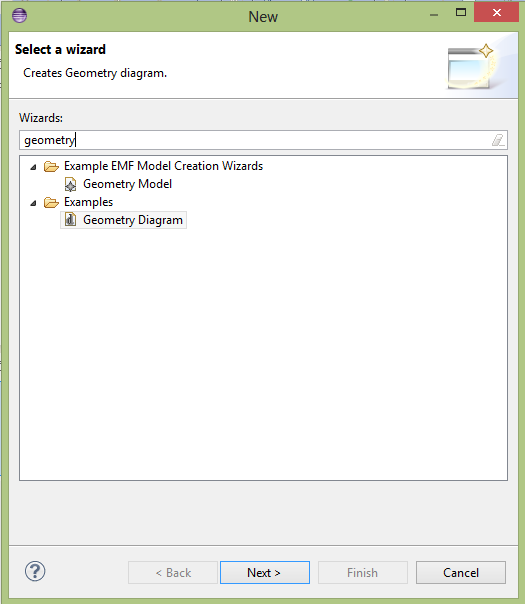
\includegraphics[width=0.8\textwidth]{image/geometry1.png}
  \caption{Use cases for the Petri net Editor}
  \label{fig:geometry1}
\end{center}
\end{figure}

\begin{figure}[htp]
\begin{center}
  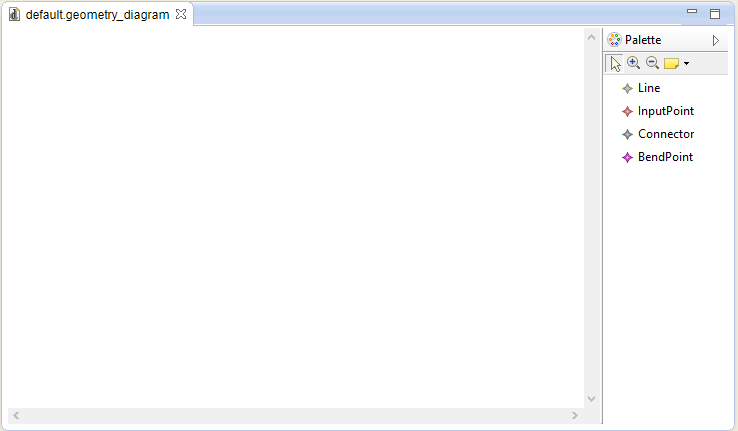
\includegraphics[width=0.8\textwidth]{image/geometry2.png}
  \caption{Use cases for the Petri net Editor}
  \label{fig:geometry2}
\end{center}
\end{figure}

\begin{figure}[htp]
\begin{center}
  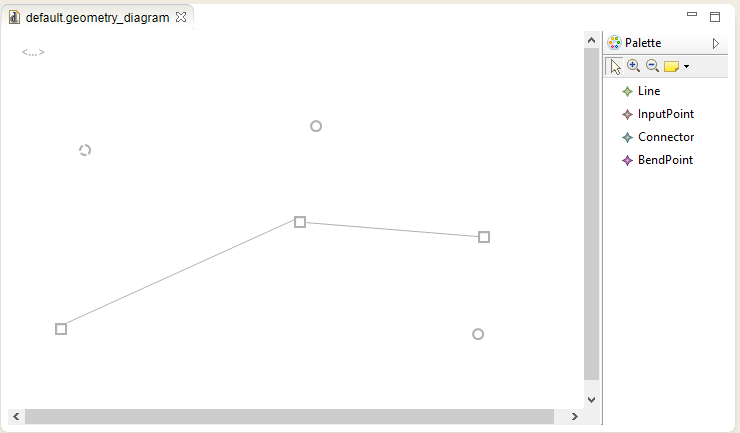
\includegraphics[width=0.8\textwidth]{image/geometry3.png}
  \caption{Use cases for the Petri net Editor}
  \label{fig:geometry3}
\end{center}
\end{figure}

\begin{figure}[htp]
\begin{center}
  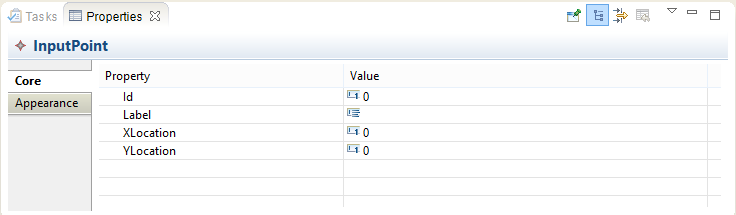
\includegraphics[width=0.8\textwidth]{image/geometry4.png}
  \caption{Use cases for the Petri net Editor}
  \label{fig:geometry4}
\end{center}
\end{figure}

\begin{figure}[htp]
\begin{center}
  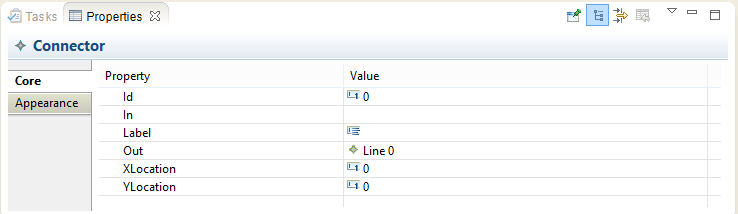
\includegraphics[width=0.8\textwidth]{image/geometry5.png}
  \caption{Use cases for the Petri net Editor}
  \label{fig:geometry5}
\end{center}
\end{figure}

\begin{figure}[htp]
\begin{center}
  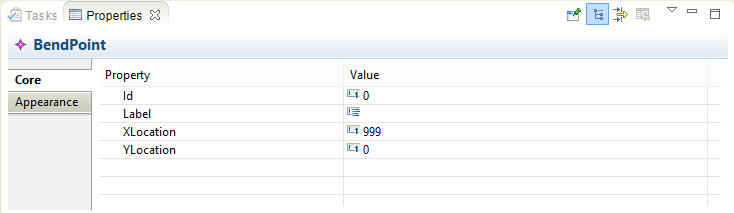
\includegraphics[width=0.8\textwidth]{image/geometry6.png}
  \caption{Use cases for the Petri net Editor}
  \label{fig:geometry6}
\end{center}
\end{figure}

\begin{figure}[htp]
\begin{center}
  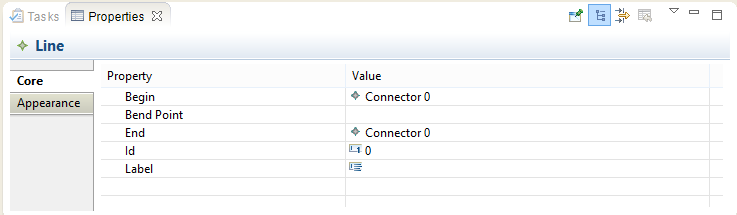
\includegraphics[width=0.8\textwidth]{image/geometry7.png}
  \caption{Use cases for the Petri net Editor}
  \label{fig:geometry7}
\end{center}
\end{figure}

Name it and click finish. On the project explorer leaf click on the file that you just generated. Geometry editor should open if it wasn’t open already.

Available tools are presented on right of the canvas. Clicking InputPoint, Connector or BendPoint allows user to create different points on the canvas. Line allows connecting Connector with each other. Following picture illustrates one example created with these tools.

Furthermore InputPoint (solid circle), Connector (box) and Bendpoints (dashed circle) can be created when user hovers the mouse on the screen for a while. A view opens which allows picking point type. Additionally hovering the mouse on a Connector presents arrows. By clicking them user can draw line to another connector the same way with clicking Line from tool palette.
Clicking on some geometry object show a property view. If this is not visible right click on a geometry object on canvas and click Show Properties View.
InputPoint has following properties to edit: Id, In, Label, Out, XLocation and YLocation. Id is a number, Label is name of the object if user wants to name it and XLocation and YLocation are the locations to show where the object is. As of currently location of canvas hasn’t anything to do with the location in the canvas. This will be adjusted on later versions of this project.

Connector has following properties to edit: Id, Label, XLocation and YLocation. Besides Id, Label and XLocation and YLocation Connector has In and Out selector. For these user can choose a Line to be connected. The number at the end of Line denotes Id.

BendPoint has the same properties as InputPoint has. The XLocation of this BendPoint has been changed to some other value.

Line has following properties to edit: Begin, BendPoint, End, Id and Label. Begin denotes the starting connector of the line. Bend Point is the parameter point on how the line is curved. The geometry canvas doesn’t show this curvature  on current version. End is the ending connector of the line.